\documentclass[aspectratio=169]{beamer}

\usepackage[T1]{fontenc}
\usepackage[utf8]{inputenc}
\usepackage{amsmath}
\usepackage{mathtools}
\usepackage{graphicx}

\usepackage{lmodern}
\usepackage{bookman}
\usecolortheme{seahorse}
\usefonttheme[onlymath]{serif}

\newenvironment{mybox}{
  \begin{beamercolorbox}[sep=0pt,center,shadow=true,rounded=true]{title}
}{
  \end{beamercolorbox}
}

\AtBeginSection[]{
  \begin{frame}
    \vfill
    \centering
    \begin{beamercolorbox}[sep=8pt,center,shadow=true,rounded=true]{title}
      \usebeamerfont{title}\insertsectionhead\par%
    \end{beamercolorbox}
    \vfill
  \end{frame}
}

\title{Slides in Latex}
\author{Markus Pawellek}

\begin{document}
  \frame{\titlepage}

  \begin{frame}{Outline}
    \footnotesize
    \hfill\parbox[t][7cm][l]{0.9\textwidth}{\tableofcontents}
  \end{frame}

  \section{Introduction}
    \begin{frame}{Introduction}
      \begin{itemize}
        \item first one
        \pause
        \item second one
        \pause
        \item third one
      \end{itemize}
    \end{frame}

  \section{Background}
    \begin{frame}{Background}
      \begin{mybox}
        \[
          \sum_{i=i}^n i = \frac{n(n+1)}{2}
        \]
      \end{mybox}
    \end{frame}

  \section{Results}
    \begin{frame}{Results}
      \begin{figure}
        \center
        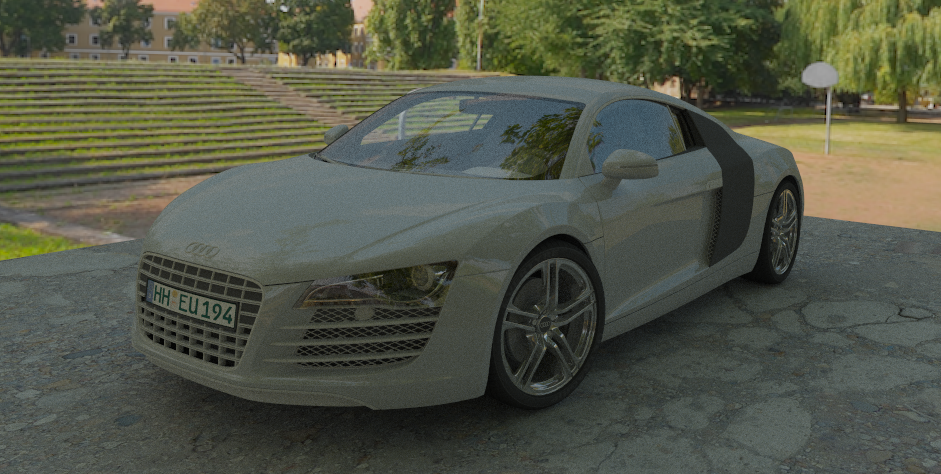
\includegraphics[height=0.7\textheight]{example-audi_r8-pt.png}
      \end{figure}
    \end{frame}

  \section{Conclusion}
    \begin{frame}{Conclusion}
      \begin{table}[H]
        \caption{Test table}
        \center
        \begin{tabular}{rrrr}
          \hline
          $x$ & $e^x$ & $\sin x$ & $\cos x$ \\
          \hline
          \hline
          $0$ & $1$ & $0$ & $1$ \\
          $1$ & $e$ & $\sin(1)$ & $\cos(1)$ \\
          $2$ & $e^2$ & $\sin(2)$ & $\cos(2)$ \\
          $3$ & $e^3$ & $\sin(3)$ & $\cos(3)$ \\
          \hline
        \end{tabular}
      \end{table}
    \end{frame}
\end{document}
